\documentclass[a4paper, fontsize = 14pt]{article}
\usepackage{hyperref}
\usepackage[warn]{mathtext}
\usepackage[english,russian]{babel}
\usepackage[utf8x]{inputenc} 
 
%математика
\usepackage[mathscr]{eucal}
\usepackage{amsmath,amsfonts,amssymb,amsthm,mathtools}
\usepackage{icomma}
\usepackage{wasysym}
\usepackage{mathrsfs}
 
%оформление текста
\usepackage{setspace}
\onehalfspacing
\usepackage{indentfirst}
\usepackage{scrextend}
 
%геометрия
\usepackage{geometry}
\geometry{left=25mm,right=25mm,
 top=25mm,bottom=30mm}
 
%графика
\usepackage{wrapfig}
\usepackage{graphicx}
\usepackage{pgfplots}
\usepackage{tikz}
\RequirePackage{caption}
\DeclareCaptionLabelSeparator{defffis}{ --- }
\captionsetup{justification=centering,labelsep=defffis}
	\usepackage{float}    %Плавающие картинки
	\usepackage{wrapfig}  %Обтекание фигур (таблиц, картинок и прочего)
	\usepackage{fancyhdr} %Загрузим пакет
 
%таблицы
\usepackage{array,tabularx,tabulary,booktabs} 
\usepackage{longtable}  
\usepackage{multirow} 
 
%ссылки
\usepackage{hyperref}
\usepackage{xcolor}
\definecolor{grn}{HTML}{57A14F} %зеленый
\definecolor{rd}{HTML}{E53C44} %красный 
\definecolor{bl}{HTML}{282691} %синий 
\definecolor{bbl}{HTML}{001B6C} %темно-синий
\hypersetup{        
    colorlinks=true,        
    linkcolor=bbl,          % внутренние ссылки
    citecolor=rd,          % на библиографию
    filecolor=magenta,      % на файлы
    urlcolor=bl           %внешние источники
}
 
	\usepackage{graphicx}
	
	\usepackage{titlesec}
	\titlelabel{\thetitle.\quad}

	\usepackage{hyperref}
	\newenvironment{comment}{}{}

%%%Конец библиотек

%%%Настройка ссылок
	\hypersetup
	{
		colorlinks = true,
		linkcolor  = blue,
		filecolor  = magenta,
		urlcolor   = blue
	}
%%%Конец настройки ссылок


%%%Настройка колонтитулы
	\pagestyle{fancy}
	\fancyhead{}
	\fancyhead[L]{3.2.5}
	\fancyhead[R]{Старченко Иван, группа Б01-005}
	\fancyfoot[C]{\thepage}
%%%конец настройки колонтитулы
 
\begin{document}

\begin{center}
  \LARGE{Лабораторная работа 3.2.5}\\[0.2cm]
  \LARGE{Вынужденные колебания в электрическом контуре.}\\[0.2cm]
  \large{5 ноября 2021 г.}\\[0.2cm]
  \large{Старченко Иван Александрович}\\[0.2cm]
\end{center}

\textbf{Цель работы:} исследование вынужденных колебаний и процессов их установления в колебательном контуре.
\\

\textbf{Оборудование:} генератор звуковых частот, вольтметр, частотомер, конденсатор, катушка индуктивности, магазин сопротивлений, осциллограф, универсальный измеритель импеданса (LCR-метр).


\section{Теоретическая справка}
\par Рассмотрим процессы, протекающие в колебательном контуре, подсоединённом к внешней ЭДС. Для колебаний в контуре имеем, применяя метод комплексных амплитуд: 
$$ \overset{\,\,..}{I} + 2\gamma \overset{\,\,.}{I}+\omega^2 I = -\varepsilon \frac{\Omega}{L} sin (\Omega t)   \Leftrightarrow  \overset{ \,\,..}{\widehat{I}} + 2\gamma \overset{\,\,.}{\widehat{I} } + \omega^2 I = -\varepsilon \frac{\Omega}{L} e^{i\Omega t} $$


\par Общим решением данного уравнения является суперпозиция синусоид: первая -- с частотой собственных колебаний контра $ \omega $ и амплитудой, экспоненциально убывающей со временем; вторая -- с частотой внешнего источника $ \Omega $ и постоянной амплитудой. Cо временем собственные колебания затухают, и в контуре устанавливаются вынужденные колебания. Амплитуда этих колебаний максимальна при совпадении частоты $ \Omega $ внешнего сигнала с собственной частотой контура $ \omega_0 $. 

\[ I = B e^{-\gamma t} sin(\omega t -\theta) + \frac{\varepsilon_0 \Omega}{L \rho_0} sin(\Omega t -\psi) \]


Резонансная частота контура определяется по формуле 
\begin{equation}
    \nu_0 = \frac{1}{2\pi \sqrt{LC}}
\end{equation}

Построив \textit{резонансные кривые} - графики зависимости $U/U_0 = f (\nu / \nu_0)$, определим добротность контура при сопротивлении $R = 0,01$ Ом и $R = 100,01$ Ом по формуле 
\begin{equation}
    Q = \frac{\nu_0}{2\triangle \nu},
\end{equation}
    где $\nu_0$ - резонансная частота, а $2\triangle \nu$ - ширина резонансной кривой при $U/U_0 = \frac{1}{\sqrt{2}}$ 
    
Также добротность колебательного контура можно установить по скорости нарастания амплитуды вынужденных колебаний при резонансе или по скорости затухания свободных колебаний. Наблюдать эти явления на осциллографе можно, если на контур подаются цуги. Чем выше добротность, тем медленнее нарастают и медленнее затухают колебания в контуре.
Логарифмический декремент затухания связан с добротностью и при исследовании затухания колебаний может быть вычислен по формуле 
\begin{equation}
    \Theta = \frac{\pi}{Q} = \frac{1}{n} ln \frac{U_k}{U_{k+n}},
\end{equation}
а при установлении колебаний в контуре
\begin{equation}
    \Theta = \frac{\pi}{Q} = \frac{1}{n} ln \frac{U_0 - U_k}{U_0 - U_{k+n}}
\end{equation}
\section{Экспериментальная установка}
Схема установки для исследования вынужденных колебаний приведена на Рис. $\ref{fig:vac}$ 
\begin{figure}[h]
    \centering
    \includegraphics[width=10cm]{fig1.PNG}
    \caption{Схема экспериментальной установки для исследования вынужденных колебаний}
    \label{fig:vac}
\end{figure}

Колебательный контур состоит из ёмкости $C = 0,1$ мкФ, индуктивности $L = 100$  мГн и переменного сопротивления $R$ \par
Также учтём достаточно большое сопротивление магазина индуктивностей и уточним фактическую его индуктивность
\begin{center}
    $R_L = 30,418$ Ом \hspace{1cm} $L = 100,4$ мГн
\end{center}

Погрешность магазинов индуктивностей и сопротивлений
\begin{center}
    $\sigma_L = 0.2008\%$ \hspace{1cm} $\sigma_R = 0,02\%$
\end{center}
\section{Ход работы}
\begin{table}[h!]
\centering
\begin{tabular}{cccccccccccc}
\hline
\multicolumn{1}{|c|}{U, В} & \multicolumn{1}{c|}{12}   & \multicolumn{1}{c|}{13}   & \multicolumn{1}{c|}{14}   & \multicolumn{1}{c|}{15}   & \multicolumn{1}{c|}{16}   & \multicolumn{1}{c|}{17}   & \multicolumn{1}{c|}{18}   & \multicolumn{1}{c|}{19}   & \multicolumn{1}{c|}{20}   & \multicolumn{1}{c|}{21}   & \multicolumn{1}{c|}{22}    \\ \hline
\multicolumn{1}{|c|}{\nu, Гц} & \multicolumn{1}{c|}{1484} & \multicolumn{1}{c|}{1490} & \multicolumn{1}{c|}{1494} & \multicolumn{1}{c|}{1499} & \multicolumn{1}{c|}{1503} & \multicolumn{1}{c|}{1507} & \multicolumn{1}{c|}{1510} & \multicolumn{1}{c|}{1514} & \multicolumn{1}{c|}{1516} & \multicolumn{1}{c|}{1518} & \multicolumn{1}{c|}{1521}  \\ \hline
\multicolumn{12}{l}{}                                                                                                                                                                                                                                                                                                                        \\ \hline
\multicolumn{1}{|c|}{U, В} & \multicolumn{1}{c|}{23}   & \multicolumn{1}{c|}{24}   & \multicolumn{1}{c|}{25}   & \multicolumn{1}{c|}{26}   & \multicolumn{1}{c|}{27}   & \multicolumn{1}{c|}{28}   & \multicolumn{1}{c|}{29}   & \multicolumn{1}{c|}{29,5} & \multicolumn{1}{c|}{30}   & \multicolumn{1}{c|}{30,5} & \multicolumn{1}{c|}{30,75} \\ \hline
\multicolumn{1}{|c|}{\nu, Гц} & \multicolumn{1}{c|}{1523} & \multicolumn{1}{c|}{1526} & \multicolumn{1}{c|}{1528} & \multicolumn{1}{c|}{1531} & \multicolumn{1}{c|}{1534} & \multicolumn{1}{c|}{1536} & \multicolumn{1}{c|}{1539} & \multicolumn{1}{c|}{1541} & \multicolumn{1}{c|}{1543} & \multicolumn{1}{c|}{1546} & \multicolumn{1}{c|}{1550}  \\ \hline
\multicolumn{12}{l}{}                                                                                                                                                                                                                                                                                                                        \\ \hline
\multicolumn{1}{|c|}{U, В} & \multicolumn{1}{c|}{30,5} & \multicolumn{1}{c|}{30}   & \multicolumn{1}{c|}{29,5} & \multicolumn{1}{c|}{29}   & \multicolumn{1}{c|}{28,5} & \multicolumn{1}{c|}{28}   & \multicolumn{1}{c|}{27}   & \multicolumn{1}{c|}{26}   & \multicolumn{1}{c|}{25}   & \multicolumn{1}{c|}{24}   & \multicolumn{1}{c|}{23}    \\ \hline
\multicolumn{1}{|c|}{\nu, Гц} & \multicolumn{1}{c|}{1551} & \multicolumn{1}{c|}{1557} & \multicolumn{1}{c|}{1559} & \multicolumn{1}{c|}{1561} & \multicolumn{1}{c|}{1563} & \multicolumn{1}{c|}{1564} & \multicolumn{1}{c|}{1566} & \multicolumn{1}{c|}{1569} & \multicolumn{1}{c|}{1572} & \multicolumn{1}{c|}{1575} & \multicolumn{1}{c|}{1577}  \\ \hline
\multicolumn{12}{l}{}                                                                                                                                                                                                                                                                                                                        \\ \hline
\multicolumn{1}{|c|}{U, В} & \multicolumn{1}{c|}{22}   & \multicolumn{1}{c|}{21}   & \multicolumn{1}{c|}{20}   & \multicolumn{1}{c|}{19}   & \multicolumn{1}{c|}{18}   & \multicolumn{1}{c|}{17}   & \multicolumn{1}{c|}{16}   & \multicolumn{1}{c|}{15}   & \multicolumn{1}{c|}{14}   & \multicolumn{1}{c|}{13}   & \multicolumn{1}{c|}{12}    \\ \hline
\multicolumn{1}{|c|}{\nu, Гц} & \multicolumn{1}{c|}{1580} & \multicolumn{1}{c|}{1585} & \multicolumn{1}{c|}{1587} & \multicolumn{1}{c|}{1590} & \multicolumn{1}{c|}{1593} & \multicolumn{1}{c|}{1597} & \multicolumn{1}{c|}{1602} & \multicolumn{1}{c|}{1606} & \multicolumn{1}{c|}{1611} & \multicolumn{1}{c|}{1618} & \multicolumn{1}{c|}{1624}  \\ \hline
\end{tabular}
\caption{Зависимость показаний вольтметра от частоты колебаний в контуре, R = 0 Ом}
\end{table}



\begin{table}[h!]
\centering
\begin{tabular}{ccccccccccc}
\hline
\multicolumn{1}{|c|}{U, В} & \multicolumn{1}{c|}{21}   & \multicolumn{1}{c|}{22}   & \multicolumn{1}{c|}{23}   & \multicolumn{1}{c|}{24}   & \multicolumn{1}{c|}{25}   & \multicolumn{1}{c|}{26}   & \multicolumn{1}{c|}{27}   & \multicolumn{1}{c|}{28}   & \multicolumn{1}{c|}{28,5} & \multicolumn{1}{c|}{29}   \\ \hline
\multicolumn{1}{|c|}{\nu, Гц} & \multicolumn{1}{c|}{1448} & \multicolumn{1}{c|}{1457} & \multicolumn{1}{c|}{1465} & \multicolumn{1}{c|}{1472} & \multicolumn{1}{c|}{1481} & \multicolumn{1}{c|}{1489} & \multicolumn{1}{c|}{1496} & \multicolumn{1}{c|}{1506} & \multicolumn{1}{c|}{1510} & \multicolumn{1}{c|}{1515} \\ \hline
\multicolumn{1}{l}{}    & \multicolumn{1}{l}{}      & \multicolumn{1}{l}{}      & \multicolumn{1}{l}{}      & \multicolumn{1}{l}{}      & \multicolumn{1}{l}{}      & \multicolumn{1}{l}{}      & \multicolumn{1}{l}{}      & \multicolumn{1}{l}{}      & \multicolumn{1}{l}{}      & \multicolumn{1}{l}{}      \\ \hline
\multicolumn{1}{|c|}{U, В} & \multicolumn{1}{c|}{29,5} & \multicolumn{1}{c|}{30}   & \multicolumn{1}{c|}{30,5} & \multicolumn{1}{c|}{31}   & \multicolumn{1}{c|}{31,2} & \multicolumn{1}{c|}{31}   & \multicolumn{1}{c|}{30,5} & \multicolumn{1}{c|}{30}   & \multicolumn{1}{c|}{29,5} & \multicolumn{1}{c|}{29}   \\ \hline
\multicolumn{1}{|c|}{\nu, Гц} & \multicolumn{1}{c|}{1521} & \multicolumn{1}{c|}{1527} & \multicolumn{1}{c|}{1535} & \multicolumn{1}{c|}{1549} & \multicolumn{1}{c|}{1558} & \multicolumn{1}{c|}{1567} & \multicolumn{1}{c|}{1581} & \multicolumn{1}{c|}{1589} & \multicolumn{1}{c|}{1596} & \multicolumn{1}{c|}{1604} \\ \hline
\multicolumn{11}{l}{}                                                                                                                                                                                                                                                                                           \\ \hline
\multicolumn{1}{|c|}{U, В} & \multicolumn{1}{c|}{28,5} & \multicolumn{1}{c|}{28}   & \multicolumn{1}{c|}{27}   & \multicolumn{1}{c|}{26}   & \multicolumn{1}{c|}{25}   & \multicolumn{1}{c|}{24}   & \multicolumn{1}{c|}{23}   & \multicolumn{1}{c|}{22}   & \multicolumn{1}{c|}{21}   & \multicolumn{1}{c|}{20}   \\ \hline
\multicolumn{1}{|c|}{\nu, Гц} & \multicolumn{1}{c|}{1609} & \multicolumn{1}{c|}{1615} & \multicolumn{1}{c|}{1626} & \multicolumn{1}{c|}{1637} & \multicolumn{1}{c|}{1648} & \multicolumn{1}{c|}{1659} & \multicolumn{1}{c|}{1670} & \multicolumn{1}{c|}{1682} & \multicolumn{1}{c|}{1695} & \multicolumn{1}{c|}{1708} \\ \hline
\end{tabular}
\caption{Зависимость показаний вольтметра от частоты колебаний в контуре, R = 100 Ом}
\end{table}
Соберем схему изображенную на Рис. $\ref{fig:vac}$. Резонансная частота в таком контуре равна $\nu_m=\frac{1}{2\pi\sqrt{LC}}$=1591,6 Гц. Будем менять частоту и фиксировать значения вольтмера. Проведем измерения без подключенного дополнительного сопротивления и с сопротивлением R=100 Ом.

Построим резонансные кривые в координатах $U/U_m = f(\nu/\nu_m)$ (Рис. $\ref{fig:R=0}$ и $\ref{fig:R=100}$).
\begin{figure}[h!]
    \centering
    \includegraphics[width=12cm]{R=0.png}
    \caption{Резонансная кривая для цепи с сопротивлением R = 0 Ом}
    \label{fig:R=0}
\end{figure}
\begin{figure}[h!]
    \centering
    \includegraphics[width=12cm]{R=100.png}
    \caption{Резонансная кривая для цепи с сопротивлением R = 100 Ом}
    \label{fig:R=100}
\end{figure}
По формуле (2) определим добротность колебательного контура при разных значениях R:
\begin{center}
$Q_0 = \frac{\nu_0}{\triangle \nu_1} = \frac{1550}{38} = 26,271$ \\
$Q_{100} = \frac{\nu_0}{\triangle \nu_2} = \frac{1558}{144,4} = 6,924$
\end{center}

Погрешность измерения ширины резонансной кривой определим по методу наименьших квадратов (прямые на резонансных кривых до начала перегиба, $\approx$ 0,95 по оси y). 
$$\sigma_{\triangle \nu} = \frac{1}{\sqrt{n}} \sqrt{\frac{<y^2>-<y>^2}{<x^2>-<x>^2} - b^2}$$

Тогда для погрешности добротности формула
$$\sigma_Q = Q\sqrt{(\frac{\sigma_{\nu_0}}{\nu_0})^2 + (\frac{\sigma_{\triangle \nu}}{\triangle \nu})^2}$$

Окончательно получим

\begin{center}
$Q_0 =  26,271 \pm 0,231 \hspace{1cm} \epsilon_0 = 0,88\% $\\
$Q_{100} =  6,924 \pm 0,005 \hspace{1cm} \epsilon_0 = 0,07\% $

\end{center}
Определим экспериментальное значение добротности контура по формуле $Q = \frac{1}{R}\sqrt{\frac{L}{C}}$

\begin{center}
    $Q_0 = 32,93 \hspace{1cm} Q_{100} = 7,68$
\end{center}

 Подключим контур к клемме "Цуги". Установим на генераторе резонансную частоту, подберём частоту развёртки ЭО, при которой на экране укладывается один цуг колебаний. Рассчитаем добротность контура при нарастании и затухании колебаний, пользуясь формулами (3) и (4). Результаты измерения запишем в таблицы 3 - 6. Фотографии картинки на осциллографие при нарастании и затухании колебаний при разных сопротивлениях в цепи представлены на Рис. $\ref{fig:2}$ и $\ref{fig:3}$.
    
    $$ Q_{up} = \frac{\pi}{\Theta} =  \pi (\frac{1}{n} ln \frac{U_0 - U_k}{U_0 - U_{k+n}})^-^1 $$

$$ Q_{down} = \frac{\pi}{\Theta} = \pi (\frac{1}{n} ln \frac{U_k}{U_{k+n}})^-^1 $$
\begin{table}[h!]
\centering
\begin{tabular}{|c|c|c|c|c|c|c|c|c|c|}
\hline
U, дел & 0,5   & 1     & 1,4   & 1,8   & 2,2  & 2,5   & 2,6   & 2,9 & 3,4 \\ \hline
Q      & 15,84 & 15,49 & 12,81 & 10,91 & 10,8 & 15,49 & 10,76 & 6,4 & 6,8 \\ \hline
\end{tabular}
\caption{Нарастание колебаний, R=0 Ом}
\end{table}

\begin{table}[h!]
\centering
\begin{tabular}{|c|c|c|c|c|c|c|c|c|c|}
\hline
U, дел & 2,7  & 2,5   & 2,2   & 1,8   & 1,6  & 1,4   & 1,3   & 1,2   & 1,1   \\ \hline
Q      & 40,8 & 30,66 & 28,14 & 28,14 & 31,3 & 29,84 & 28,14 & 30,73 & 32,74 \\ \hline
\end{tabular}
    \caption{Затухание колебаний, R = 0 Ом}
\end{table}



\begin{table}[h!]
\centering
\begin{tabular}{|c|c|c|c|c|c|c|}
\hline
U, дел & 2,7  & 0,8  & 1,5  & 2    & 2,3  & 2,5  \\ \hline
Q      & 6,83 & 6,29 & 5,58 & 5,83 & 5,72 & 5,26 \\ \hline
\end{tabular}
    \caption{Нарастание колебаний, R = 100 Ом}
\end{table}


\begin{table}[h!]
\centering
\begin{tabular}{|c|c|c|c|c|c|c|}
\hline
U, дел & 2,3  & 1,5  & 1    & 0,7  & 0,5  & 0,3  \\ \hline
Q      & 7,35 & 7,54 & 7,92 & 8,23 & 7,74 & 8,24 \\ \hline
\end{tabular}
\caption{Затухание колебаний, R = 100 Ом}
\end{table}
    
 

Рассчитаем погрешность определения средней величины Q по формуле $$\sigma_Q = \sqrt{\frac{1}{n(n-1)}\sum(x_i - <x>)}$$

Тогда получившиеся значения добротностей для каждой серии измерений:

\begin{center}
 
    $Q_0_u_p = 12,189 \pm 12,891$ \hspace{1cm}  $\epsilon = 105,8\% $ \\
    $Q_0_d_o_w_n = 30,403 \pm 38,634$  \hspace{1cm} $\epsilon = 127,1\% $\\
    $Q_{100 up} = 5,766 \pm 1,169$ \hspace{1cm}  $ \epsilon = 20,3\% $ \\
    $Q_{100 down} = 7,925 \pm 1,133$ \hspace{1cm}  $\epsilon = 14,3\% $
\end{center}

\begin{figure}
    \centering
    \includegraphics[width=10cm]{1.jpg}
    \caption{Биения}
    \label{fig:1}
\end{figure}
\begin{figure}[h]
   
\begin{minipage}[h]{0.49\linewidth}
\center{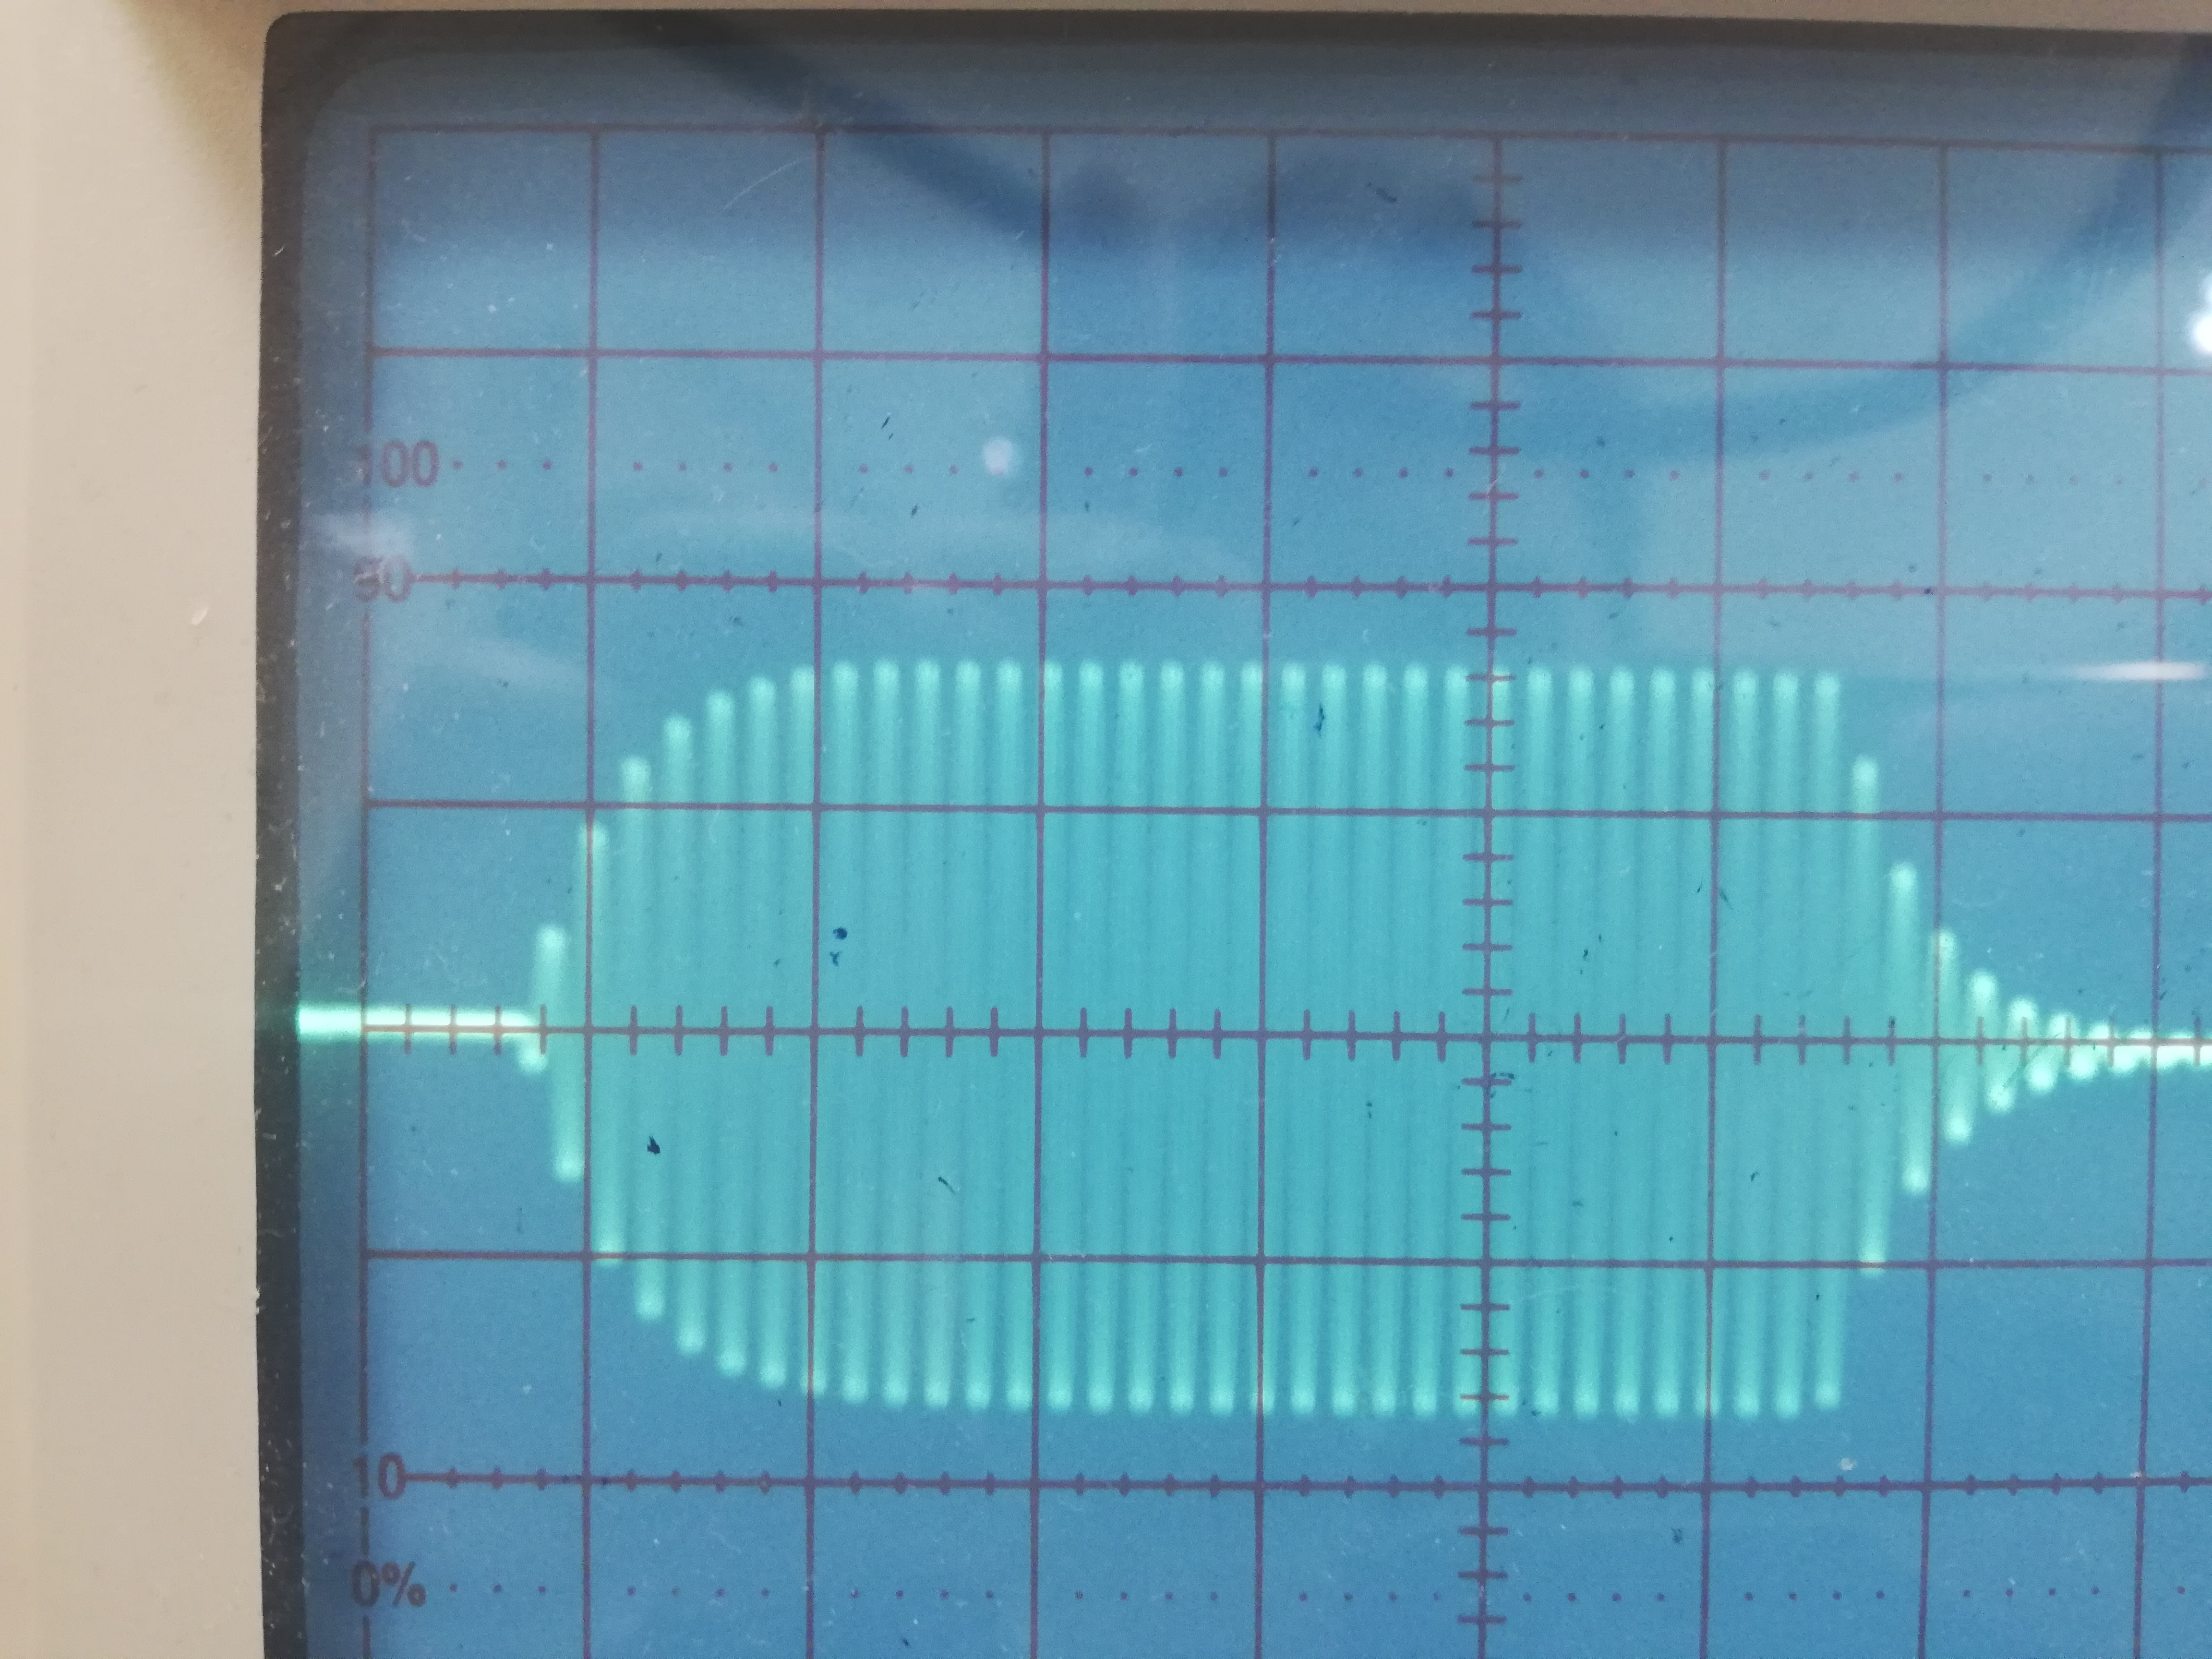
\includegraphics[width=\linewidth]{2.jpg}}
\end{minipage}
\begin{minipage}[h]{0.49\linewidth}
\center{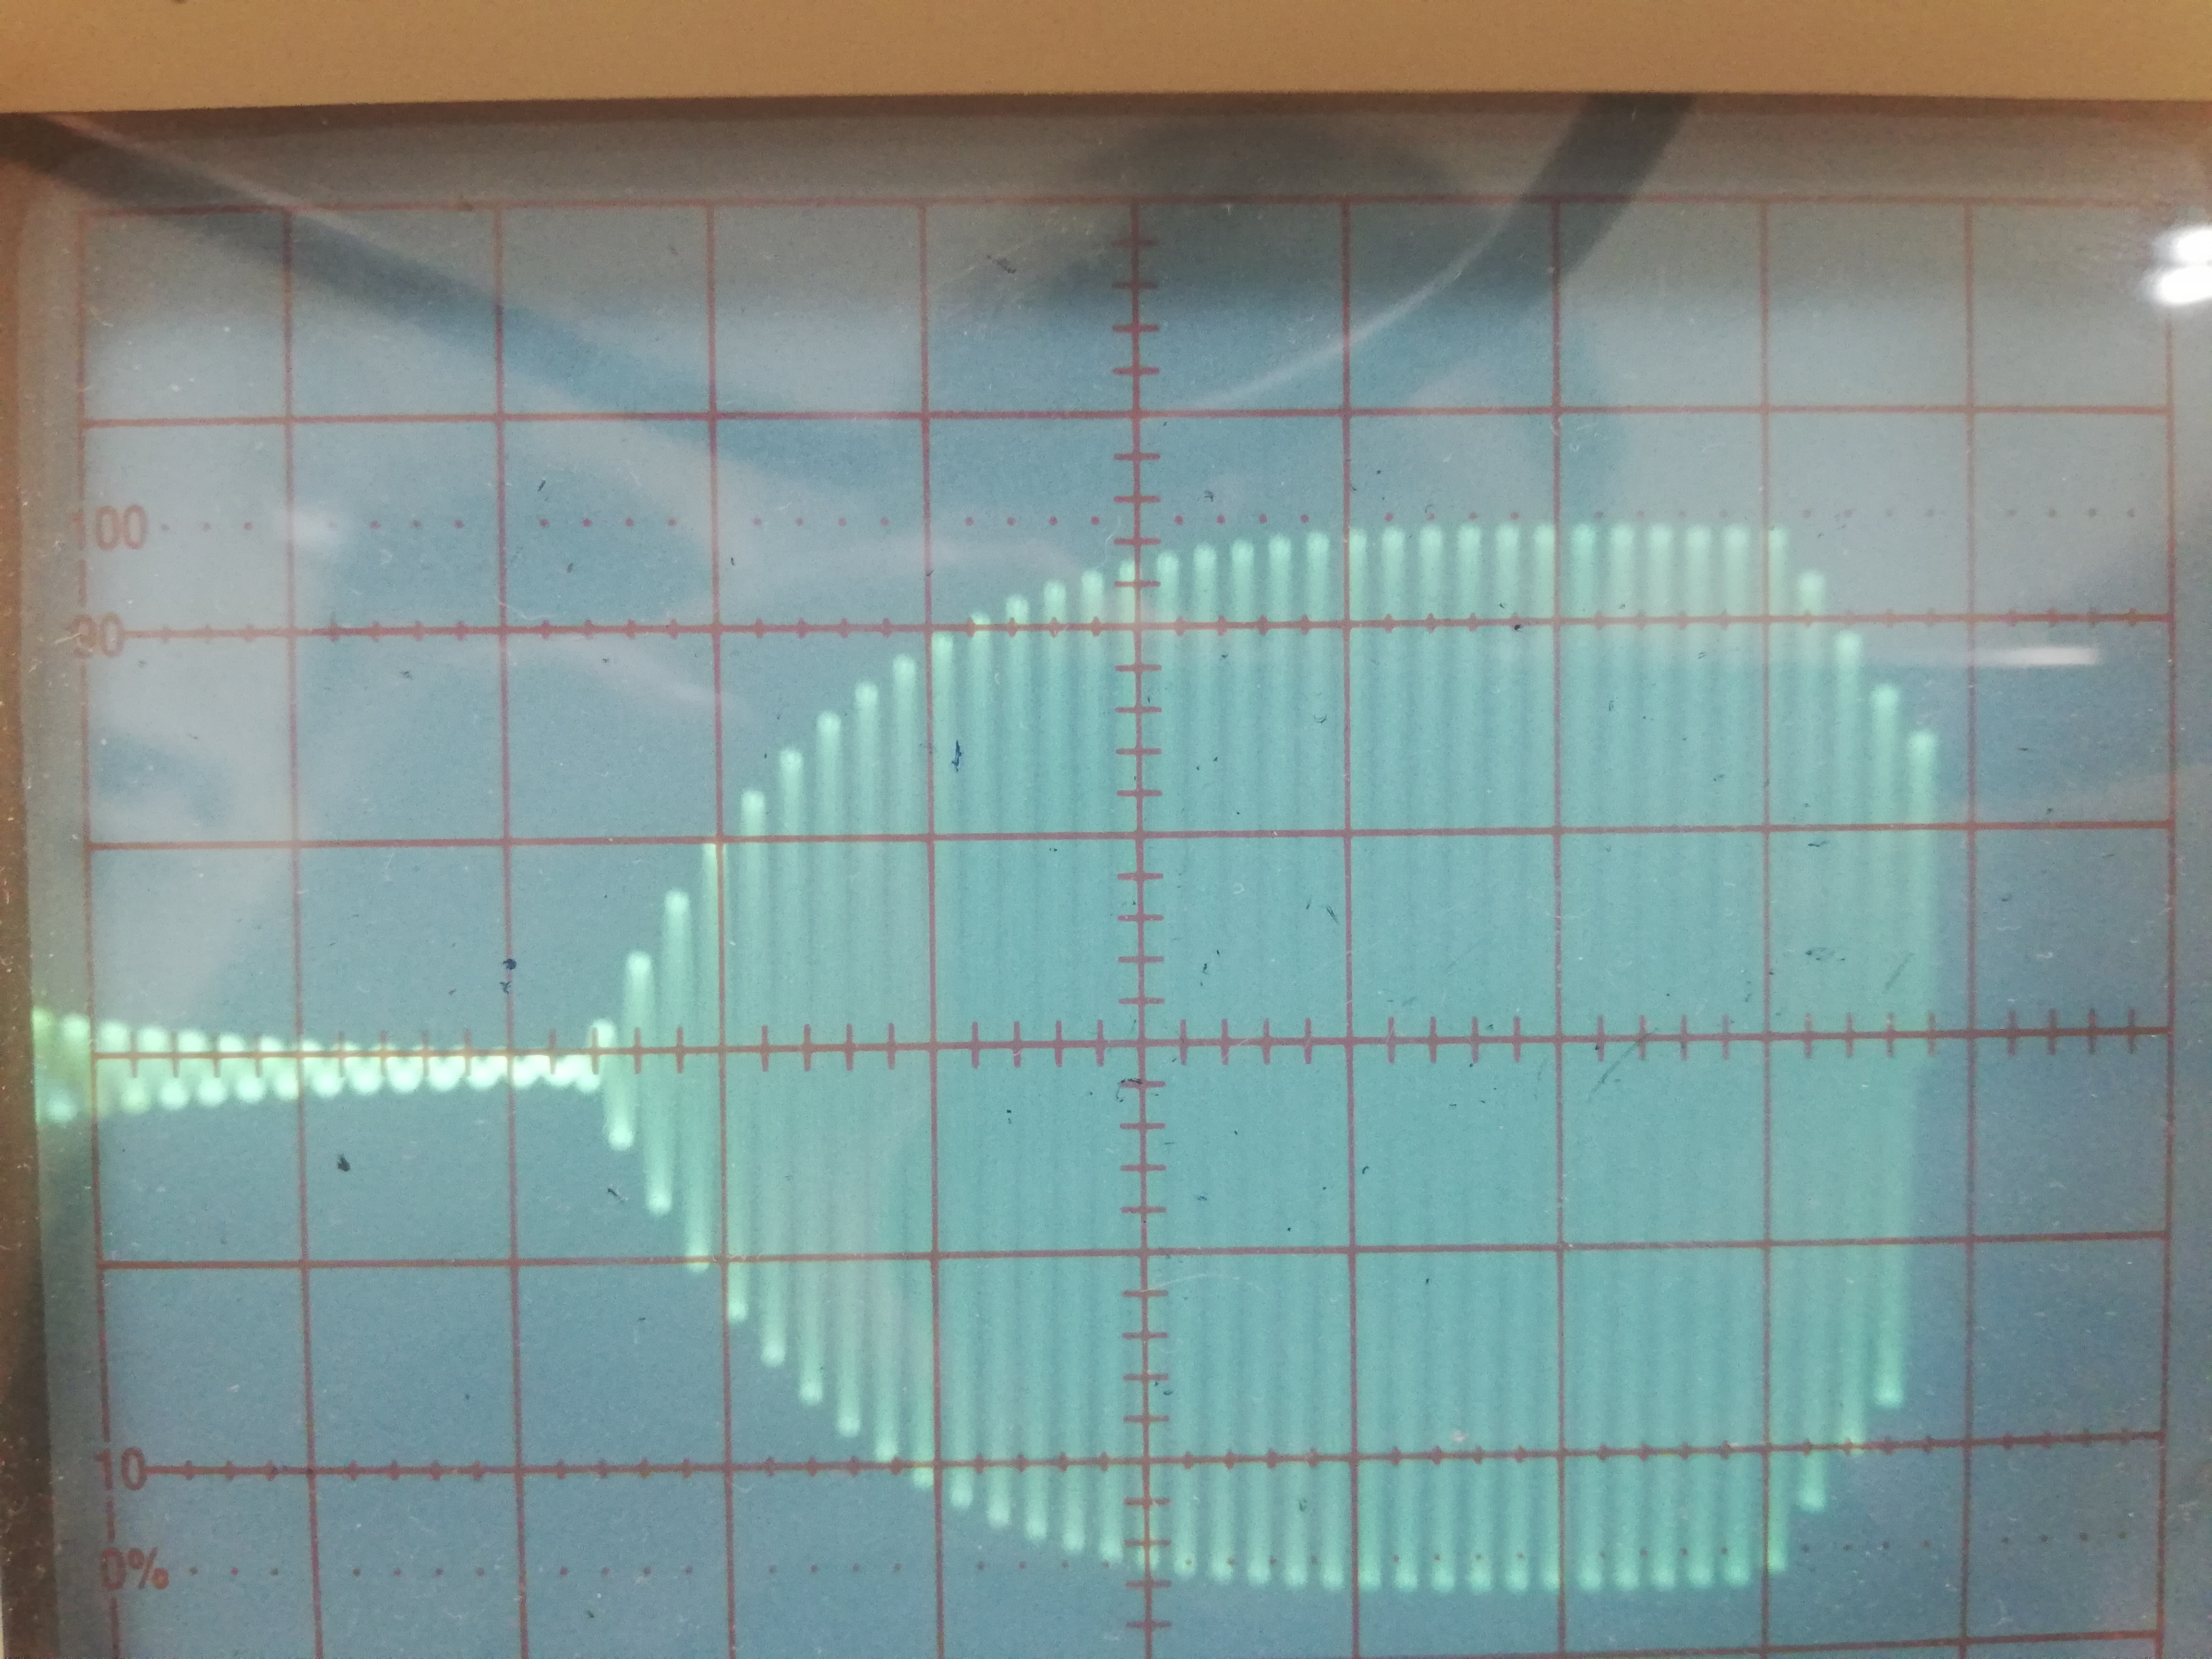
\includegraphics[width=\linewidth]{3.jpg}}
\end{minipage}
\label{fig:2}
\caption{Нарастание и затухание колебаний при R = 100 Ом}
\end{figure}
\begin{figure}[h]
   
\begin{minipage}[h]{0.49\linewidth}
\center{\includegraphics[width=\linewidth]{4.jpg}}
\end{minipage}
\begin{minipage}[h]{0.49\linewidth}
\center{\includegraphics[width=\linewidth]{5.jpg}}
\end{minipage}
\label{fig:3}
\caption{Нарастание и затухание колебаний при R = 0 Ом}
\end{figure}
\end{document}
